\apendice{Documentación de usuario}

\section{Introducción}
En esta sección, se explicará y mostrará la forma correcta de ejecutar la aplicación por parte del usuario.

\section{Requisitos de usuarios}
El usuario puede acceder a la aplicación a través del enlace: \url{https://teachmeplay.herokuapp.com/}

La aplicación se ha desplegado en Heroku, lo que significa que está siempre disponible, siempre y cuando se tenga una conexión a Internet y se disponga de un navegador compatible.

Debido a las limitaciones de Heroku en términos de tiempo de espera y almacenamiento de archivos cargados en la aplicación, la funcionalidad de carga de archivos del profesor solo estará disponible para su uso en entornos locales. Si se intenta cargar un archivo en la versión desplegada de la aplicación, se producirá un error.
Para utilizar esta función del profesor, se proporciona una máquina virtual que incluye todos los recursos necesarios para su correcto funcionamiento. Los usuarios deberán descargar y utilizar esta máquina virtual para probar la funcionalidad de carga de archivos de los juegos.

Como la aplicación consta de tres roles diferentes, se proporcionan las credenciales de tres usuarios, cada uno con un rol específico, para realizar pruebas de las distintas funcionalidades:
\begin{itemize}
    \item \textbf{Rol de usuario:} nombre de usuario ``UsuarioPruebas`` y contraseña ``UsuarioPruebas1+``.
    \item \textbf{Rol de profesor}: nombre de usuario ``ProfesorPruebas`` y contraseña ``ProfesorPruebas1+".
    \item \textbf{Rol de administrador:} nombre de usuario ``AdministradorPruebas`` y contraseña ``AdministradorPruebas1+``.
\end{itemize}

\section{Instalación}
Dado que se trata de una aplicación web, no es necesario realizar ninguna instalación adicional, ya que se puede acceder a ella a través de la URL en la que está desplegada.

En el caso de querer probar la funcionalidad para cargar archivos de los juegos se dispone de una máquina virtual.

\section{Manual del usuario}
El manual de usuario se ha realizado en una wiki disponible tanto en español como en inglés.

El manual en español está accesible a través del enlace: \url{https://ebd1004alu.gitbook.io/teachmeplay-es/}. Y, el manual en inglés está accesible a través del enlace: \url{https://ebd1004alu.gitbook.io/teachmeplay-en/}.

A continuación, se muestran los pasos a seguir para el uso de la aplicación web.

\subsection{Inicio}
Para iniciar la aplicación se accede al enlace: \url{https://teachmeplay.herokuapp.com/}.

Esta es la primera página que se muestra al acceder a la aplicación web. En ella se presentan el nombre y el logotipo de la aplicación, una breve descripción de lo que el usuario puede hacer en ella, así como el nombre y la institución de la autora.

Aquí, el usuario tiene la opción de registrarse o iniciar sesión para acceder a la aplicación. Además, puede cambiar el idioma de la aplicación a inglés o continuar en español, que es el idioma por defecto de la aplicación.

\begin{figure}[htb]
\centering
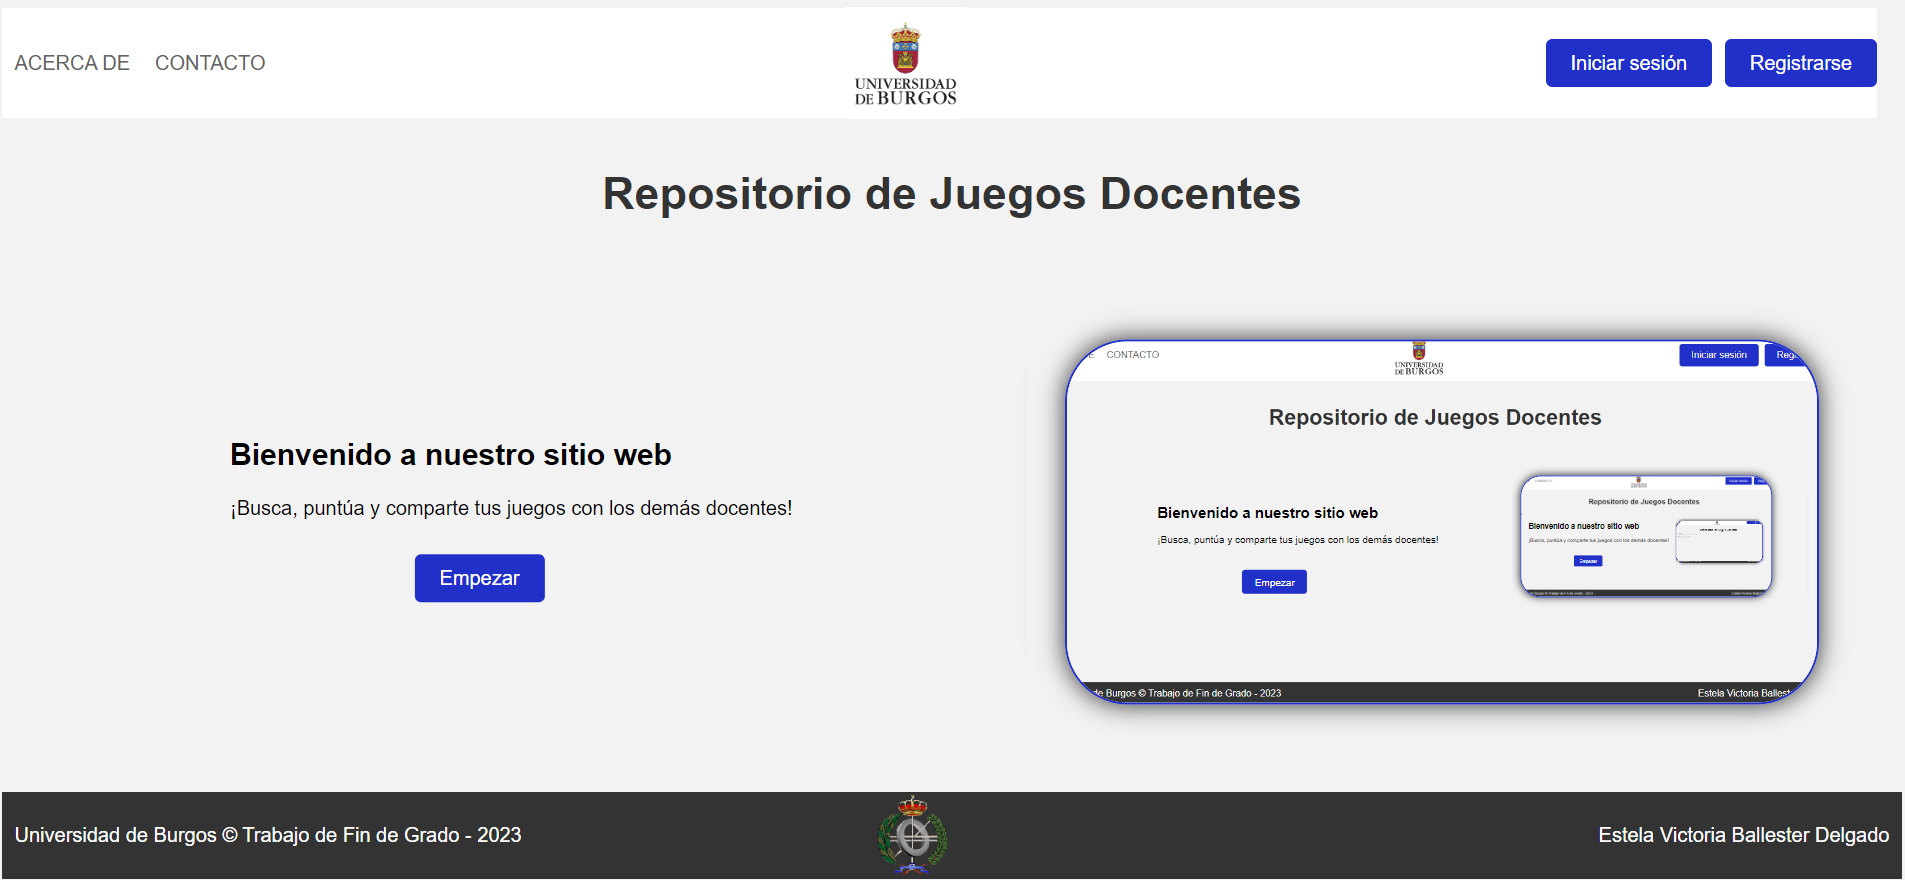
\includegraphics[width=1.0\textwidth]{inicio}
\caption{Página de inicio de la aplicación.}
\label{fig:inicio}
\end{figure}

\subsection{Acerca de}
En la sección ``Acerca de``, se presenta una breve explicación sobre el propósito y los objetivos de la aplicación.
\begin{figure}[htb]
\centering
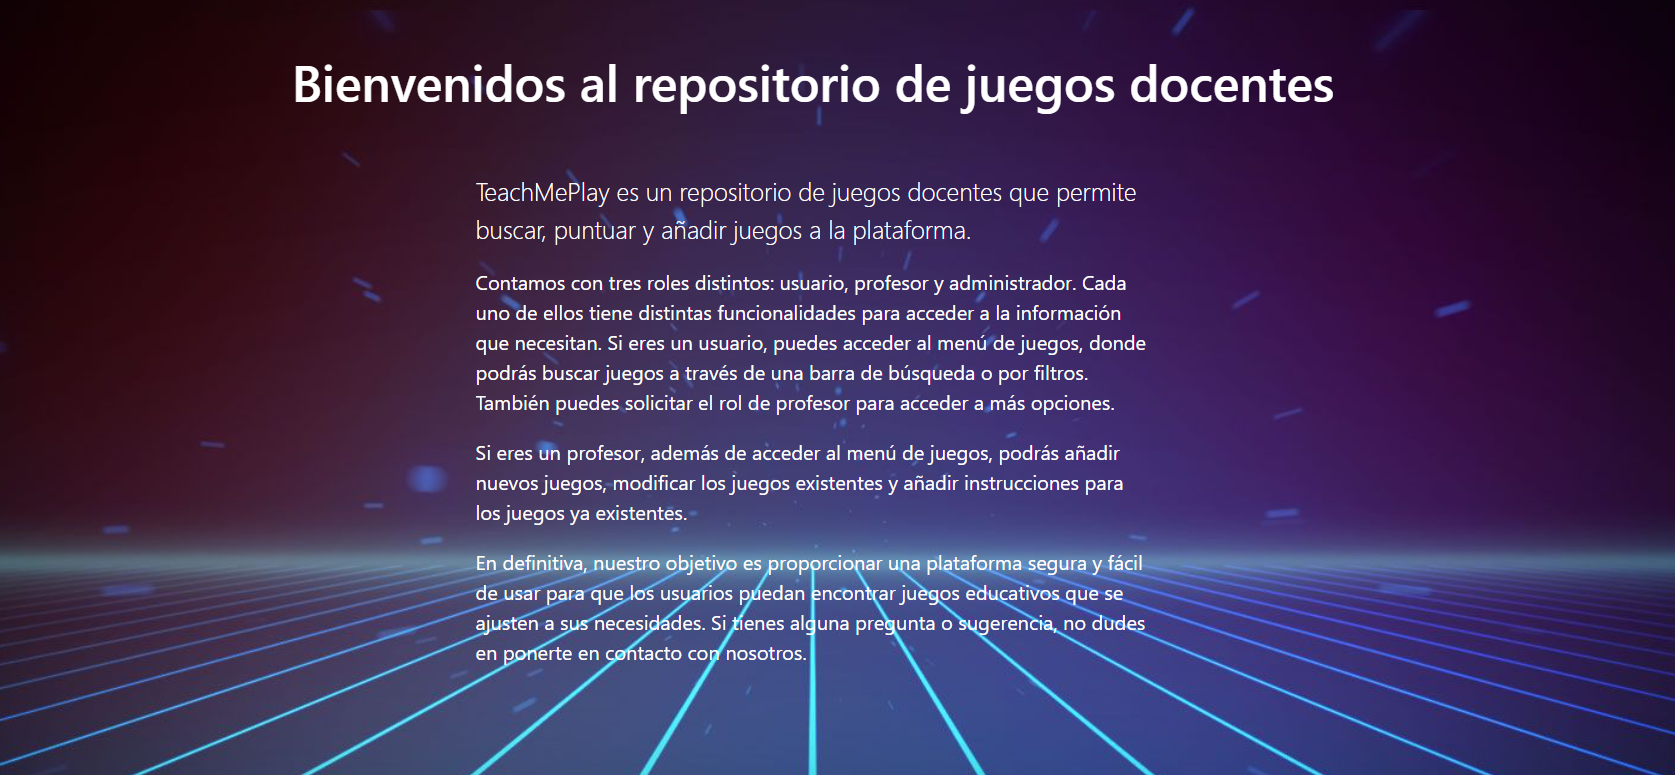
\includegraphics[width=1.0\textwidth]{acerca}
\caption{Acerca de de la aplicación.}
\label{fig:acerca}
\end{figure}

En el botón de ayuda de la cabecera de la página de inicio se abrirá el manual de ayuda para el usuario. 
\begin{figure}[htb]
\centering

\includegraphics[width=0.2\textwidth]{btn-help}
\caption{Botones de ayuda.}
\label{fig:btn-help}
\end{figure}

Si se está accediendo desde la aplicación con el idioma en español, se abrirá el manual de ayuda en español; y si se está accediendo desde la aplicación con el idioma en inglés, se abrirá el manual de ayuda en inglés.

\subsection{Iniciar sesión}
La página de iniciar sesión va a permitir acceder al menú de juegos.

\begin{figure}[htb]
\centering
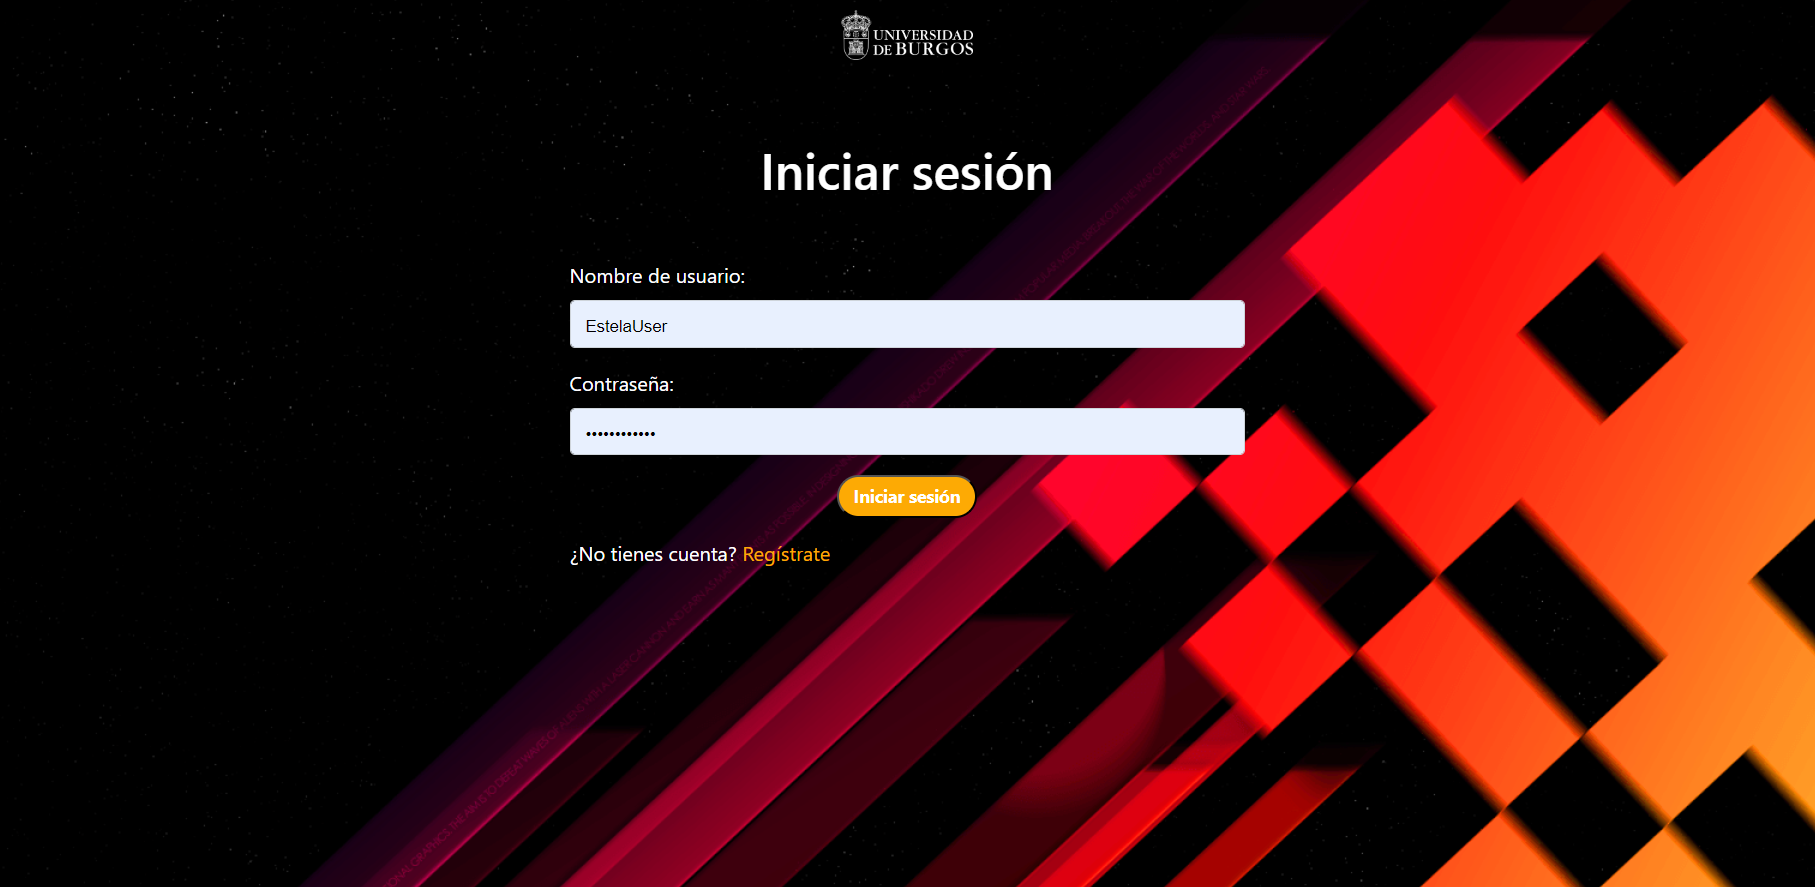
\includegraphics[width=1.0\textwidth]{login}
\caption{Página de login de la aplicación.}
\label{fig:login}
\end{figure}

Si el usuario no tiene una cuenta, se le permite registrarse a través del botón ``Registrarse``.

\begin{figure}[htb]
\centering

\includegraphics[width=0.4\textwidth]{no-cuenta}
\caption{Usuario no tiene cuenta.}
\label{fig:no-cuenta}
\end{figure}

En el caso de que el usuario ya tenga una cuenta y desee acceder a la aplicación, debe ingresar sus credenciales, es decir, su nombre de usuario y contraseña.

Si el usuario introduce incorrectamente las credenciales, se mostrará un mensaje de error indicando que las credenciales son incorrectas.
\begin{figure}[htb]
\centering
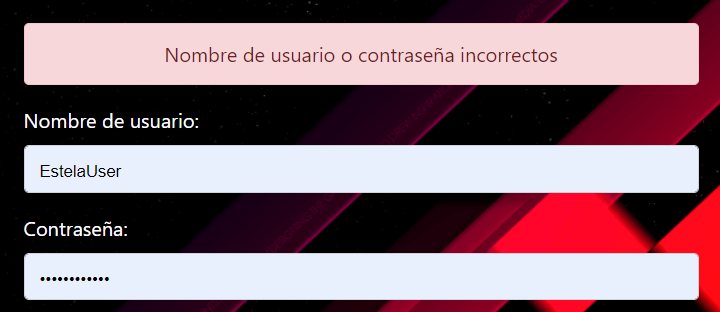
\includegraphics[width=1.0\textwidth]{incorrectos}
\caption{Nombre de usuario o contraseña incorrectos.}
\label{fig:incorrectos}
\end{figure}

Si el usuario ingresa las credenciales incorrectas tres veces, su cuenta será bloqueada durante un minuto, lo que le impedirá iniciar sesión.
\begin{figure}[htb]
\centering
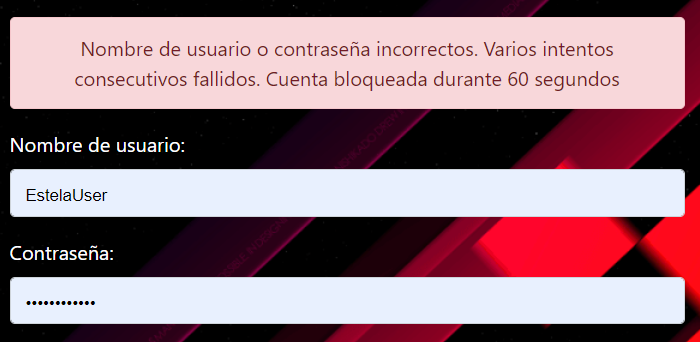
\includegraphics[width=1.0\textwidth]{bloqueada}
\caption{Varios intentos consecutivos fallidos. Cuenta bloqueada.}
\label{fig:bloqueada}
\end{figure}

Si el usuario introduce correctamente las credenciales, será redirigido al menú de juegos.

\subsection{Registrarse}
La página de registro va a permitir al usuario crearse una cuenta nueva.
\begin{figure}[htb]
\centering
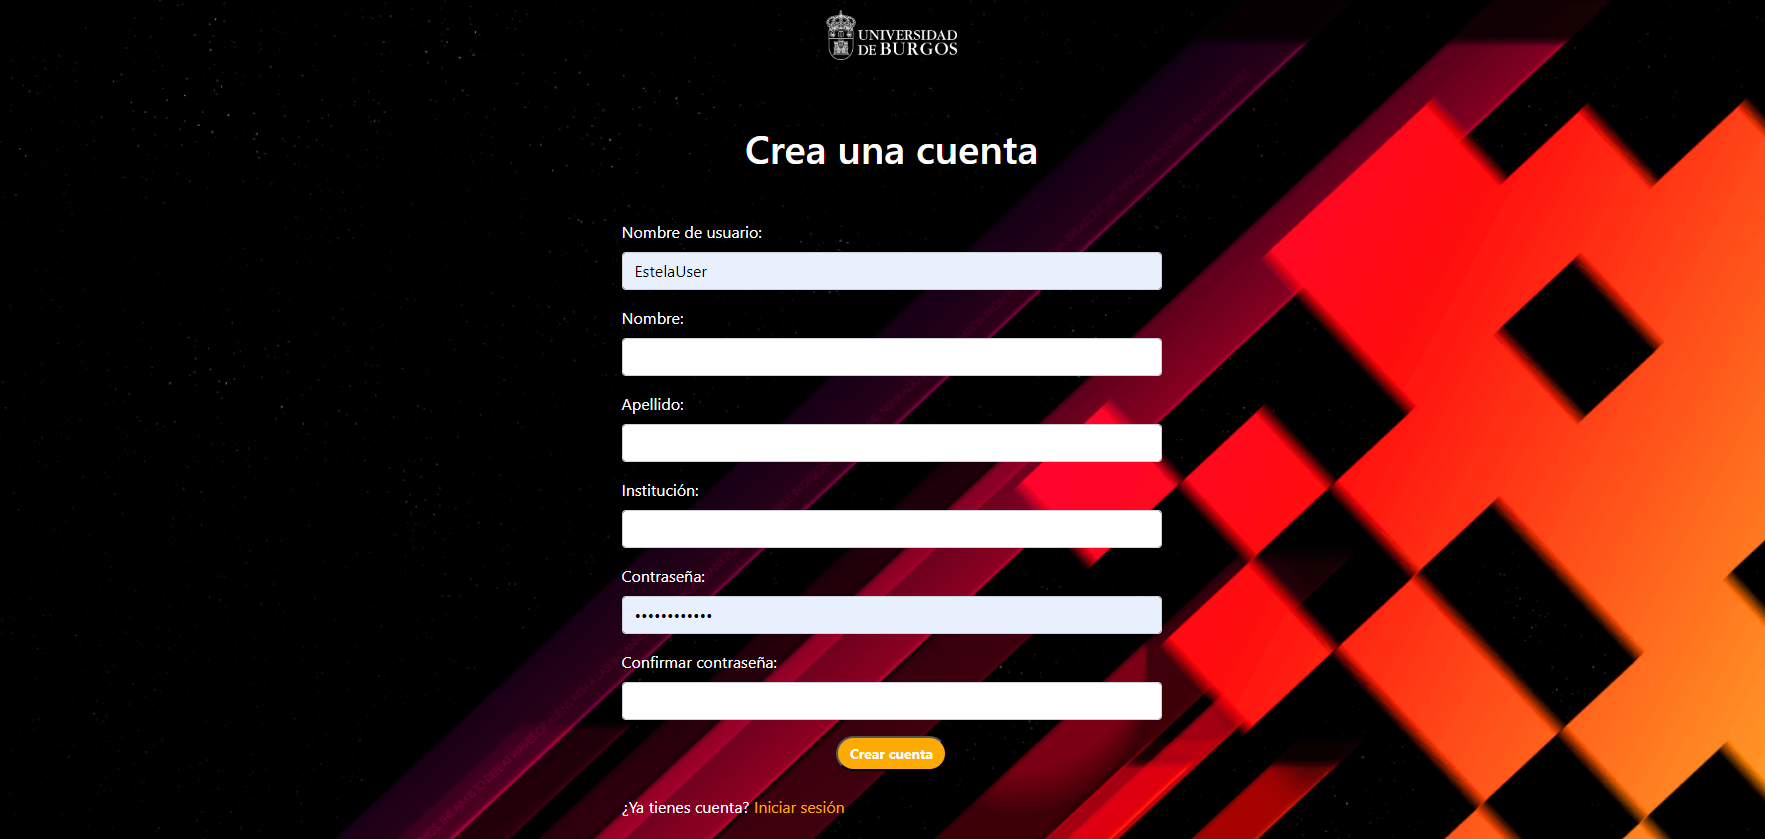
\includegraphics[width=1.0\textwidth]{registro}
\caption{Página de registro de la aplicación.}
\label{fig:registro}
\end{figure}

Si el usuario ya tiene una cuenta, se le permite iniciar sesión a través del botón ``Iniciar sesión``.

\begin{figure}[htb]
\centering

\includegraphics[width=0.4\textwidth]{ya-cuenta}
\caption{Usuario ya tiene cuenta.}
\label{fig:ya-cuenta}
\end{figure}

Para registrarse, el usuario debe completar los campos requeridos que se muestran, como el nombre de usuario, su nombre, apellido e institución. Todos estos campos son obligatorios, excepto la institución, que es opcional. Si alguno de los campos requeridos no se completa, no se permitirá completar el registro.
\newpage
\begin{figure}[htb]
\centering

\includegraphics[width=1.0\textwidth]{completa-campo}
\caption{Completa campo requerido.}
\label{fig:completa-campo}
\end{figure}

Para completar el registro, el nombre de usuario elegido por el usuario no debe estar en uso por otro usuario en la aplicación.

\begin{figure}[htb]
\centering
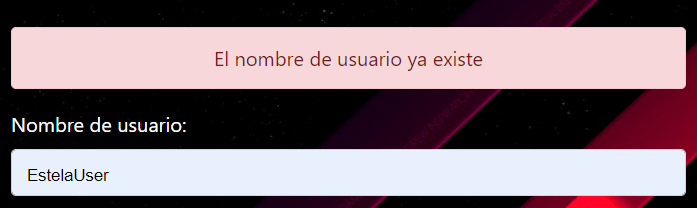
\includegraphics[width=1.0\textwidth]{existe}
\caption{Nombre de usuario ya existe.}
\label{fig:existe}
\end{figure}

Además, la contraseña debe cumplir con ciertos requisitos, como tener al menos 8 caracteres, una mayúscula y un símbolo.
\newpage
\begin{figure}[htb]
\centering
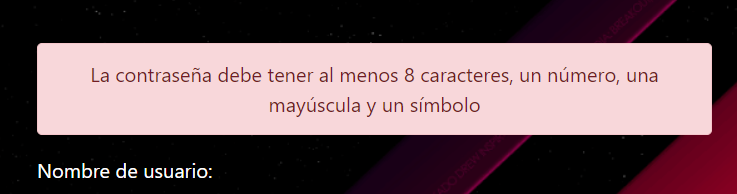
\includegraphics[width=1.0\textwidth]{condiciones}
\caption{Requisitos que la contraseña debe cumplir.}
\label{fig:condiciones}
\end{figure}

Si la contraseña y su confirmación no coinciden, se mostrará un mensaje de error.
\begin{figure}[htb]
\centering

\includegraphics[width=1.0\textwidth]{no-coinciden}
\caption{Las contraseñas no coinciden.}
\label{fig:no-coinciden}
\end{figure}

En el caso de que todos los campos sean completados correctamente y cumplan con las condiciones, el usuario será redirigido a la ventana de inicio de sesión.

\subsection{Cerrar sesión}
Todos los usuarios cuentan con un botón "Cerrar sesión" mediante el cual pueden finalizar la sesión de su cuenta. Al hacer clic en este botón, se redirigen a la página de inicio.
Si la contraseña y su confirmación no coinciden, se mostrará un mensaje de error.

\begin{figure}[htb]
\centering

\includegraphics[width=0.2\textwidth]{cerrar}
\caption{Botón cerrar sesión.}
\label{fig:cerrar}
\end{figure}
\newpage

\subsection{Menú de juegos para los usuarios}
Cuando el usuario ha iniciado sesión correctamente, se le redirige a su menú de juegos, donde puede acceder a diversas funcionalidades.
\begin{figure}[htb]
\centering
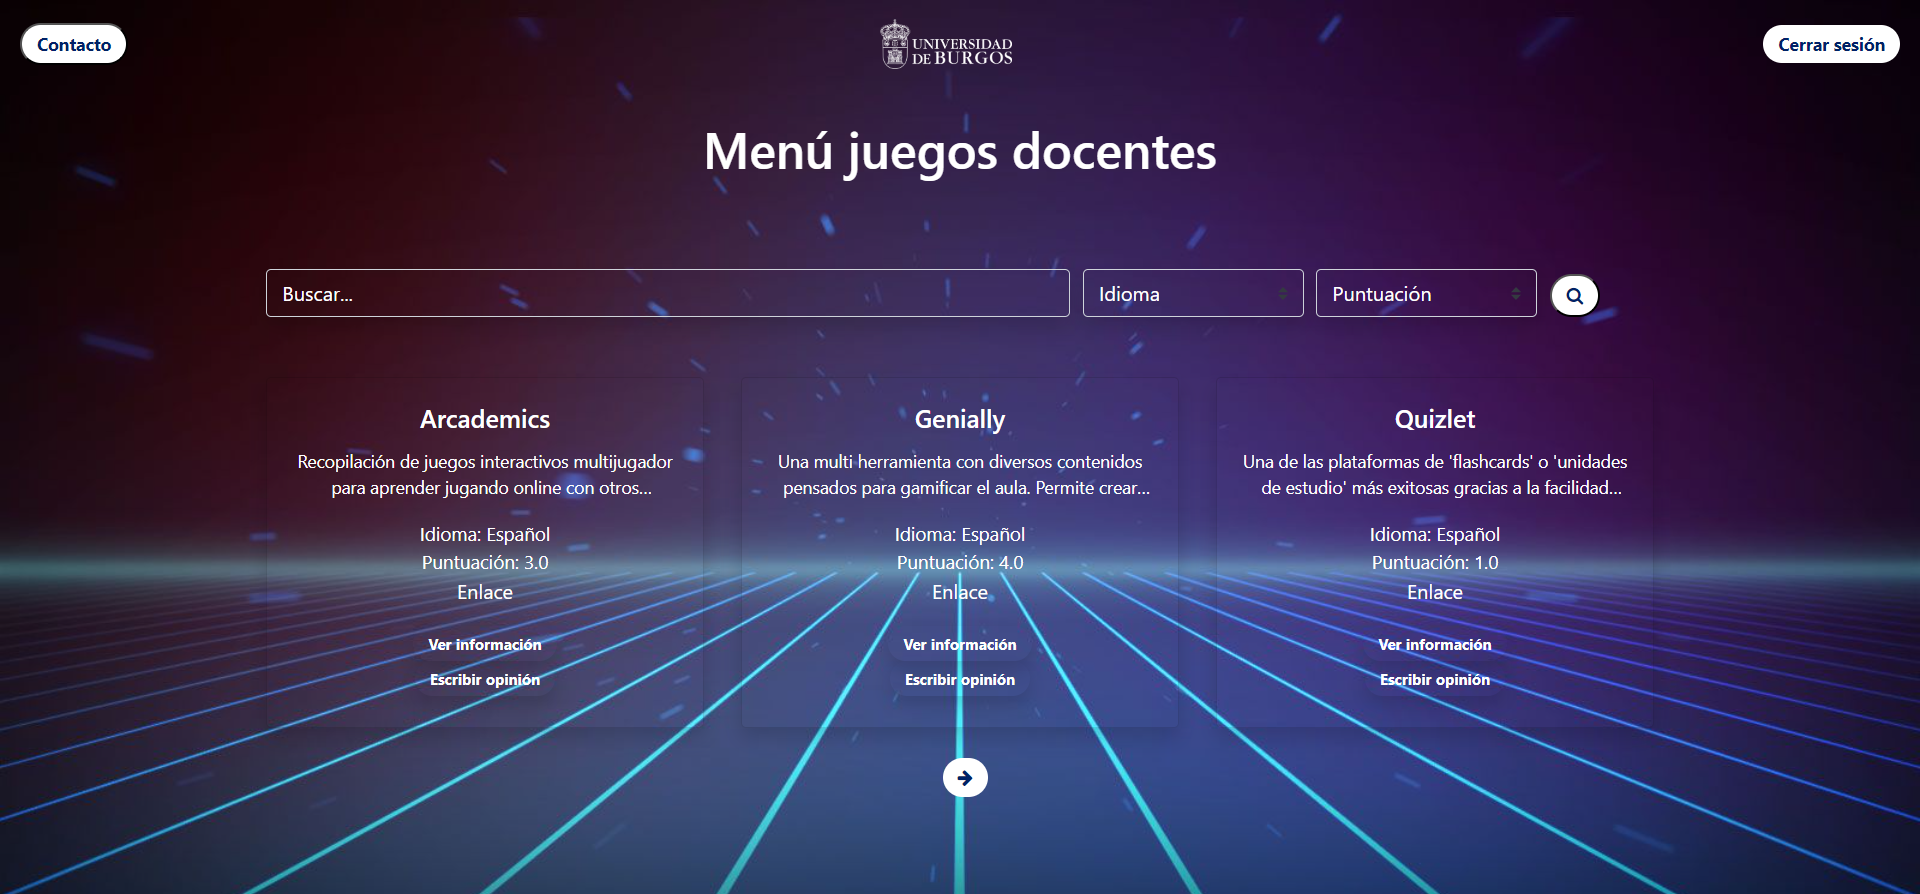
\includegraphics[width=1.0\textwidth]{menu-usuarios}
\caption{Menú de juegos de los usuarios.}
\label{fig:menu-usuarios}
\end{figure}

Principalmente, el usuario visualiza las tarjetas de información de los distintos juegos disponibles en la aplicación. Desde estas tarjetas, puede obtener más información sobre cada juego o agregar una valoración. Es importante tener en cuenta que si el usuario ya ha valorado un juego, no se le permite volver a valorarlo.
\begin{figure}[htb]
\centering
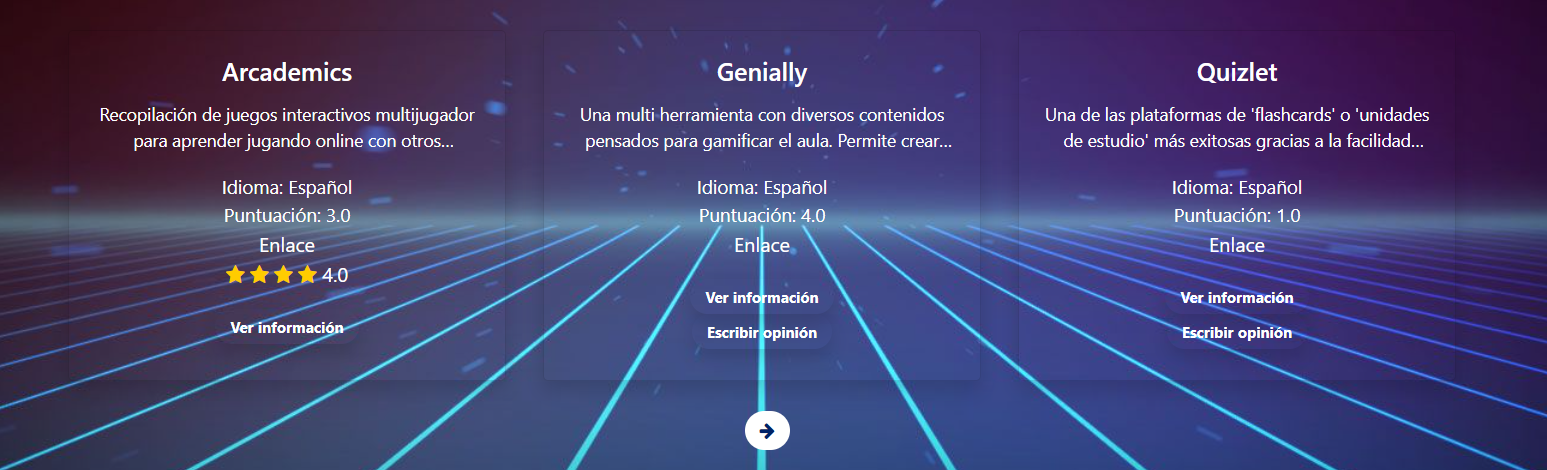
\includegraphics[width=1.0\textwidth]{tarjetas}
\caption{Tarjetas de los juegos.}
\label{fig:tarjetas}
\end{figure}

Además, el usuario cuenta con una barra de búsqueda y filtros en la aplicación, lo que le permite realizar una búsqueda personalizada y más específica según sus intereses.
\begin{figure}[htb]
\centering

\includegraphics[width=1.0\textwidth]{buscar}
\caption{Barra de búsqueda y filtros.}
\label{fig:buscar}
\end{figure}

En la cabecera, el usuario también tiene acceso a un botón llamado ``Contacto``, a través del cual puede enviar una solicitud para obtener el rol de profesor. 
\begin{figure}[htb]
\centering

\includegraphics[width=0.2\textwidth]{btn-contacto}
\caption{Botón contacto.}
\label{fig:btn-contacto}
\end{figure}

Obtener este rol ampliará las funcionalidades disponibles para el usuario en la aplicación. 

\begin{figure}[htb]
\centering

\includegraphics[width=1.0\textwidth]{btn-solicitar}
\caption{Solicitar rol de profesor.}
\label{fig:btn-solicitar}
\end{figure}

Si el usuario ya ha solicitado este rol previamente, no se le permitirá hacerlo nuevamente y se mostrará un mensaje de éxito indicando que la solicitud ya ha sido enviada. En ese caso, el usuario deberá esperar a que el administrador apruebe la solicitud.
\begin{figure}[htb]
\centering

\includegraphics[width=1.0\textwidth]{exito}
\caption{Solicitud del rol de profesor enviada con éxito.}
\label{fig:exito}
\end{figure}

\subsection{Ver más información del juego}
Para ver más información de un juego se debe pulsar al botón de ver información de la tarjeta del menú de juegos.
\begin{figure}[htb]
\centering
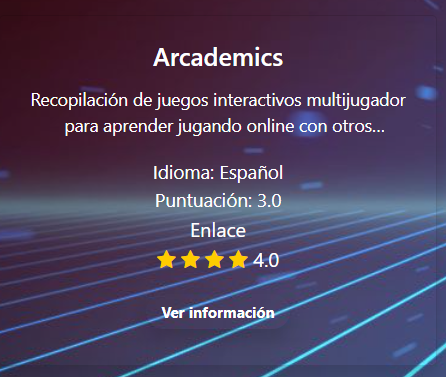
\includegraphics[width=0.5\textwidth]{btn-info}
\caption{Botón ver información de juego.}
\label{fig:btn-info}
\end{figure}

En esta ventana aparece toda la información más detallada de cada juego.
\newpage
\begin{figure}[htb]
\centering
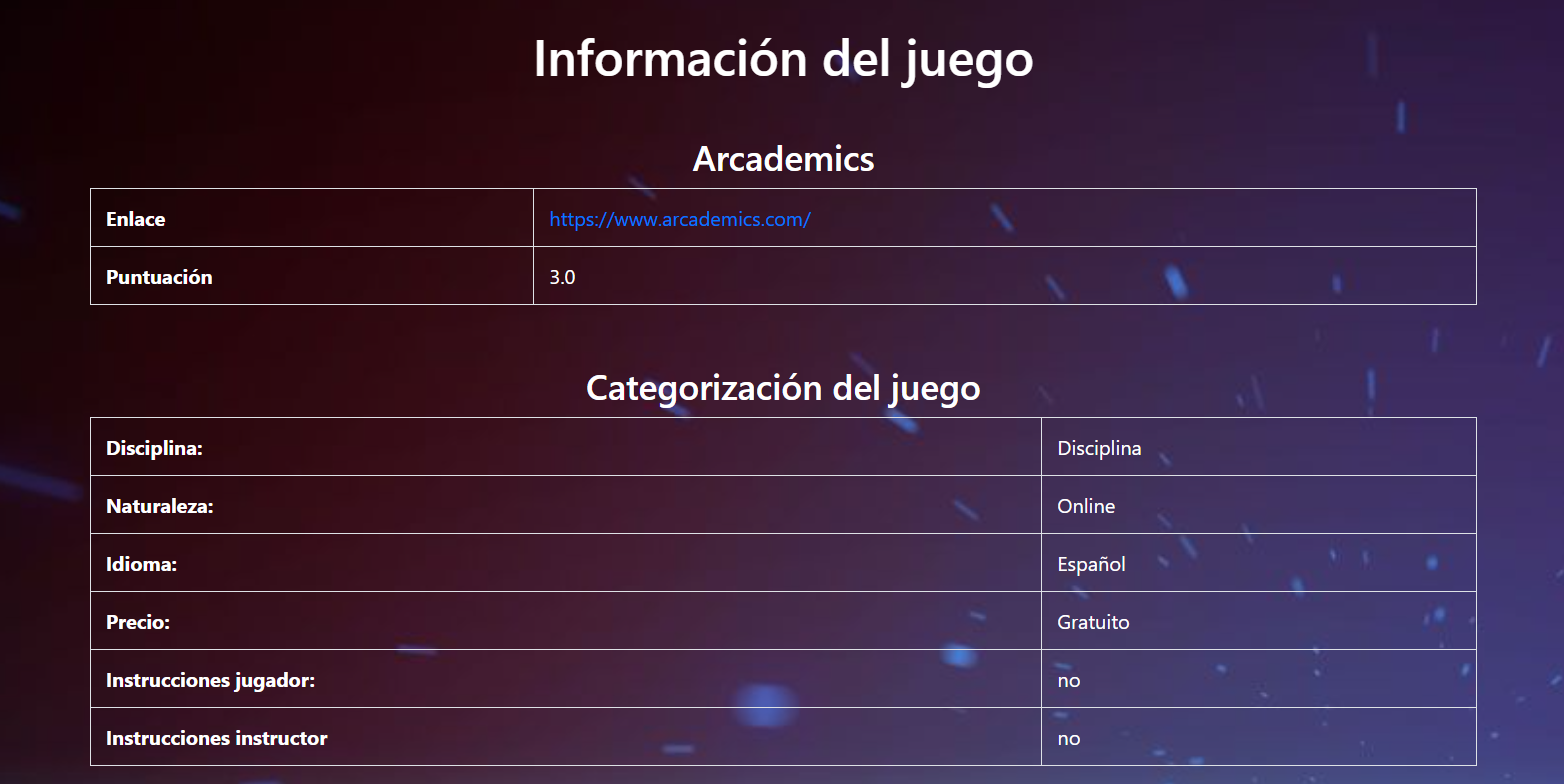
\includegraphics[width=1.0\textwidth]{informacion}
\caption{Ver información de juego.}
\label{fig:informacion}
\end{figure}

En la información del juego se le permite al usuario descargar los archivos de las instrucciones del jugador y del instructor en el caso de que se encuentren disponibles.
\begin{figure}[htb]
\centering
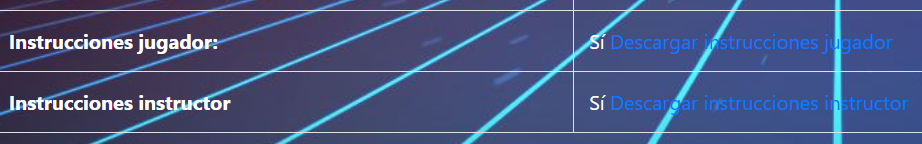
\includegraphics[width=1.0\textwidth]{descargar-archivos}
\caption{Descargar archivos de instrucciones.}
\label{fig:descargar-archivos}
\end{figure}

También, en el caso de que esté disponible el archivo del propio juego el usuario podrá descargarlo.
\begin{figure}[htb]
\centering

\includegraphics[width=1.0\textwidth]{descargar-archivo}
\caption{Descargar archivos de instrucciones.}
\label{fig:descargar-archivo}
\end{figure}

\subsection{Valorar un juego}
En esta ventana el usuario puede añadir una puntuación y un comentario a un juego.
\begin{figure}[htb]
\centering
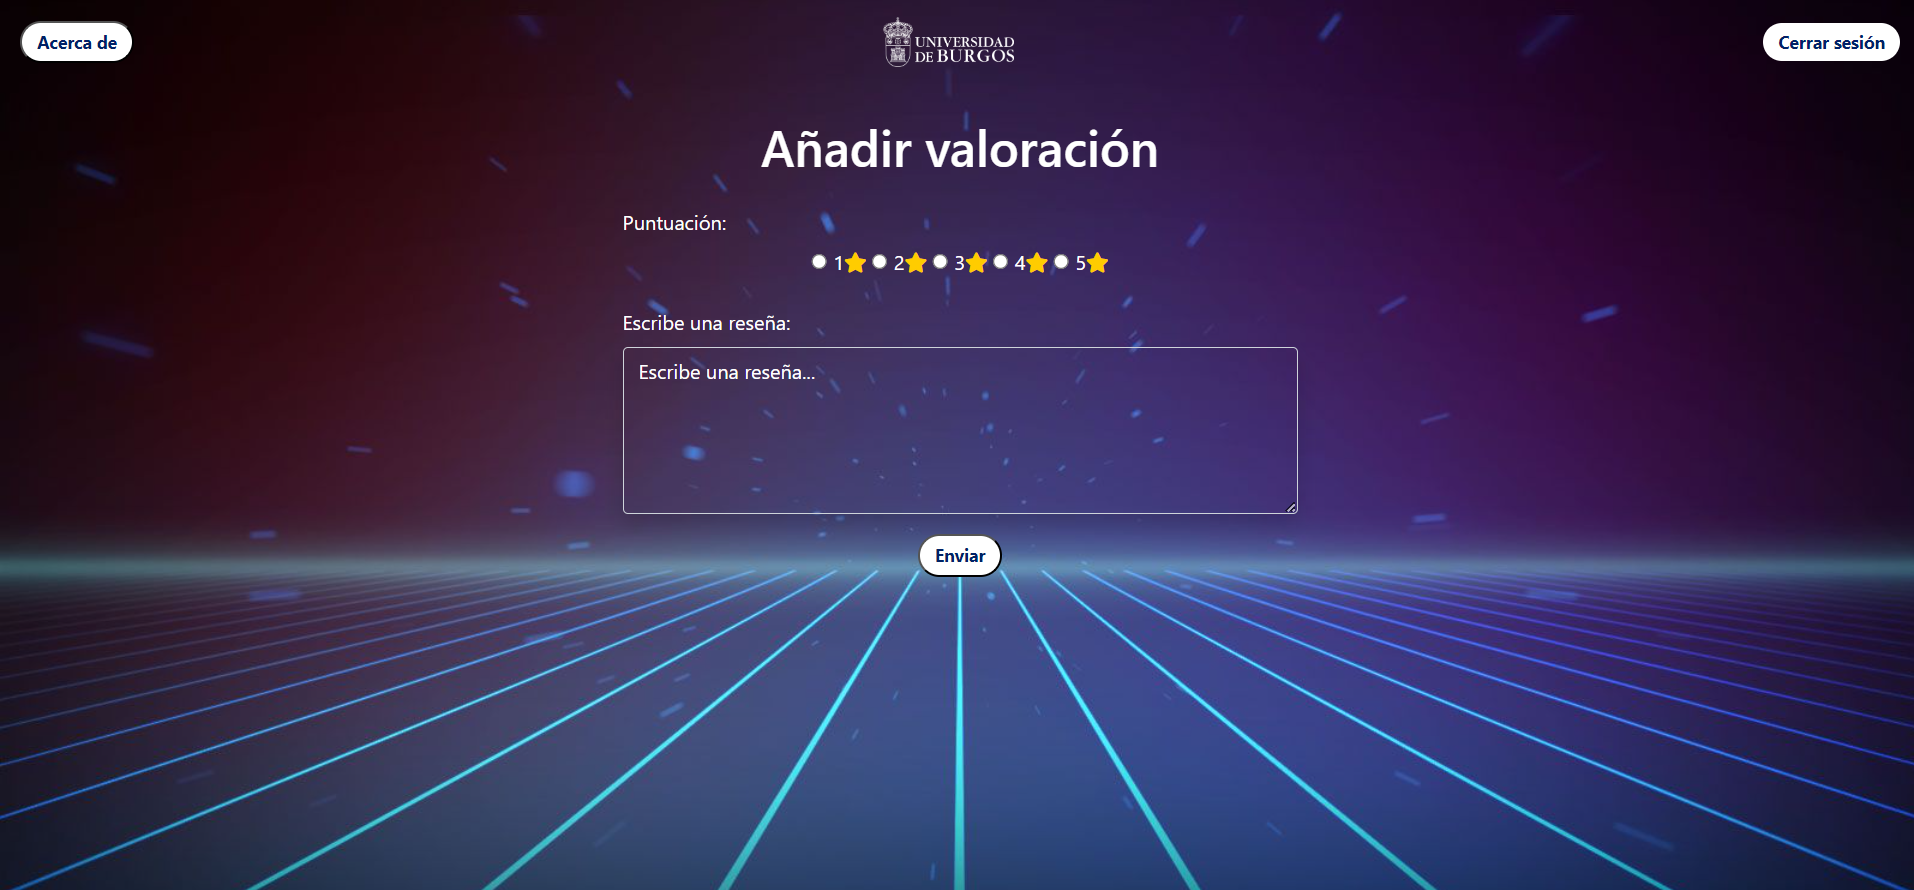
\includegraphics[width=1.0\textwidth]{añadir-valoracion}
\caption{Añadir valoración de juego.}
\label{fig:añadir-valoracion}
\end{figure}

\subsection{Visualizar valoraciones de juegos}
Para ver más todas las valoraciones que tiene un juego se debe pulsar a la puntuación que se encuentra al lado de las estrellas.
\newpage
\begin{figure}[htb]
\centering
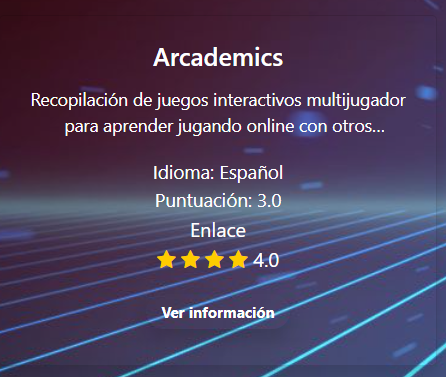
\includegraphics[width=0.5\textwidth]{btn-info}
\caption{Botón ver valoraciones de juego.}
\label{fig:btn-info}
\end{figure}

En esta ventana aparece todas las valoraciones de cada juego.
\begin{figure}[htb]
\centering
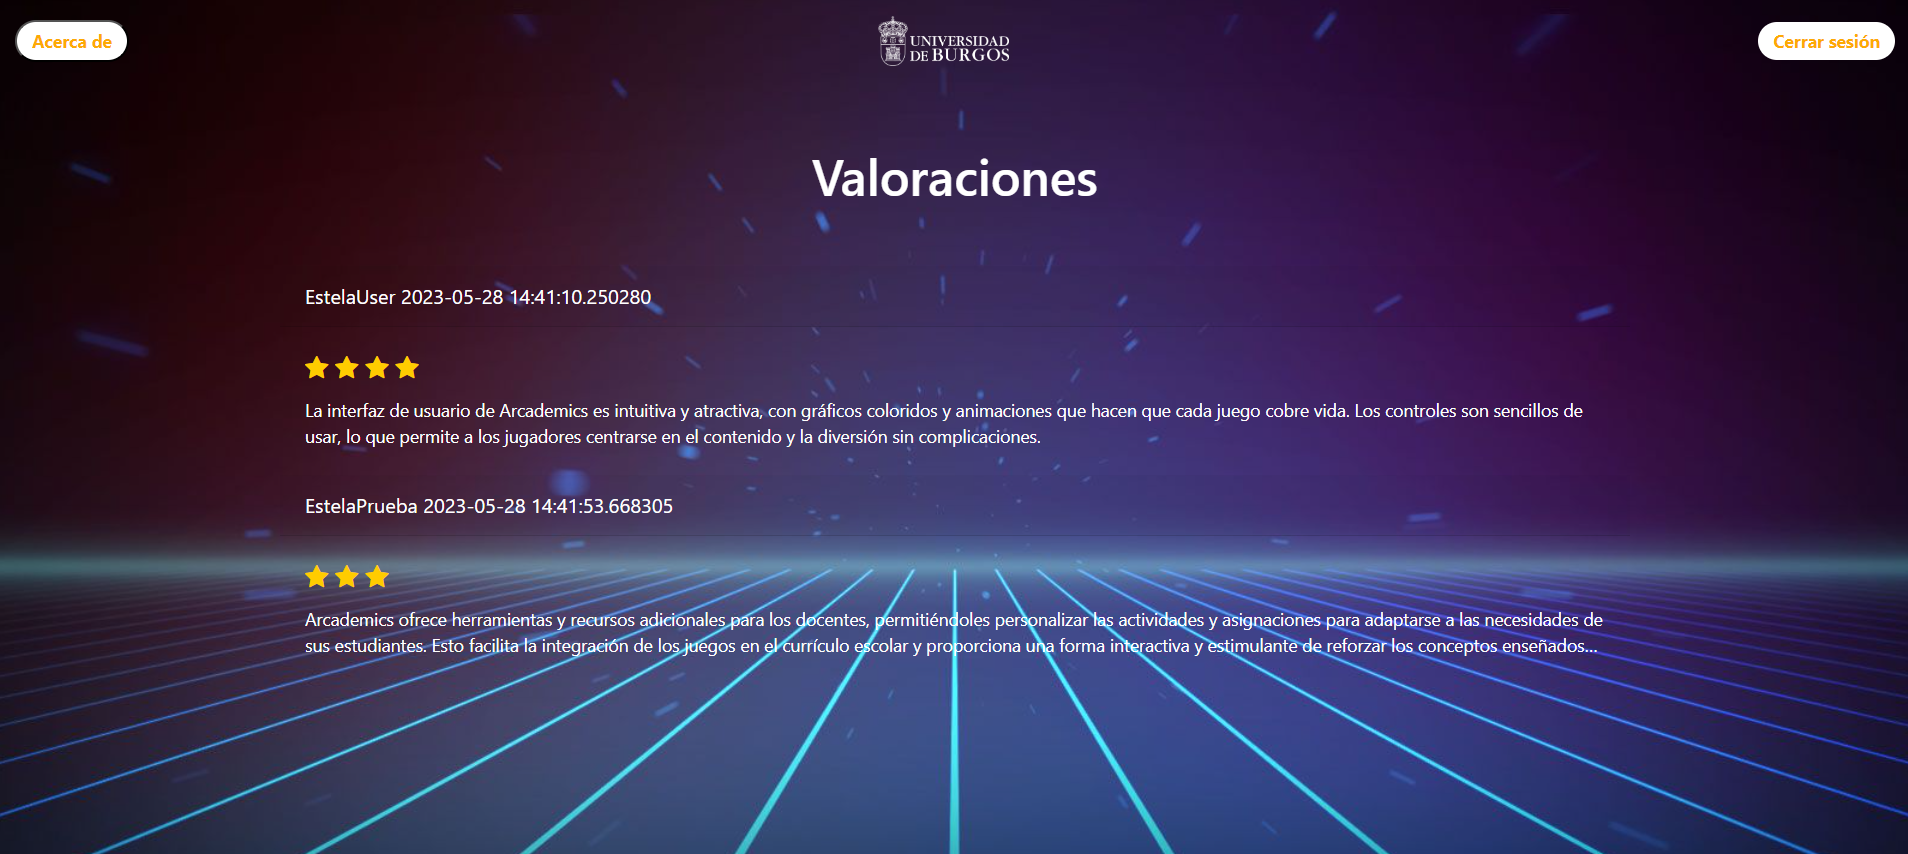
\includegraphics[width=1.0\textwidth]{visualizar-valoracion}
\caption{Visualizar valoraciones de juego.}
\label{fig:visualizar-valoracion}
\end{figure}

\subsection{Menú de juegos para los profesores}
Cuando el profesor ha iniciado sesión correctamente, se le redirige a su menú de juegos, donde puede acceder a diversas funcionalidades.
\newpage
\begin{figure}[htb]
\centering
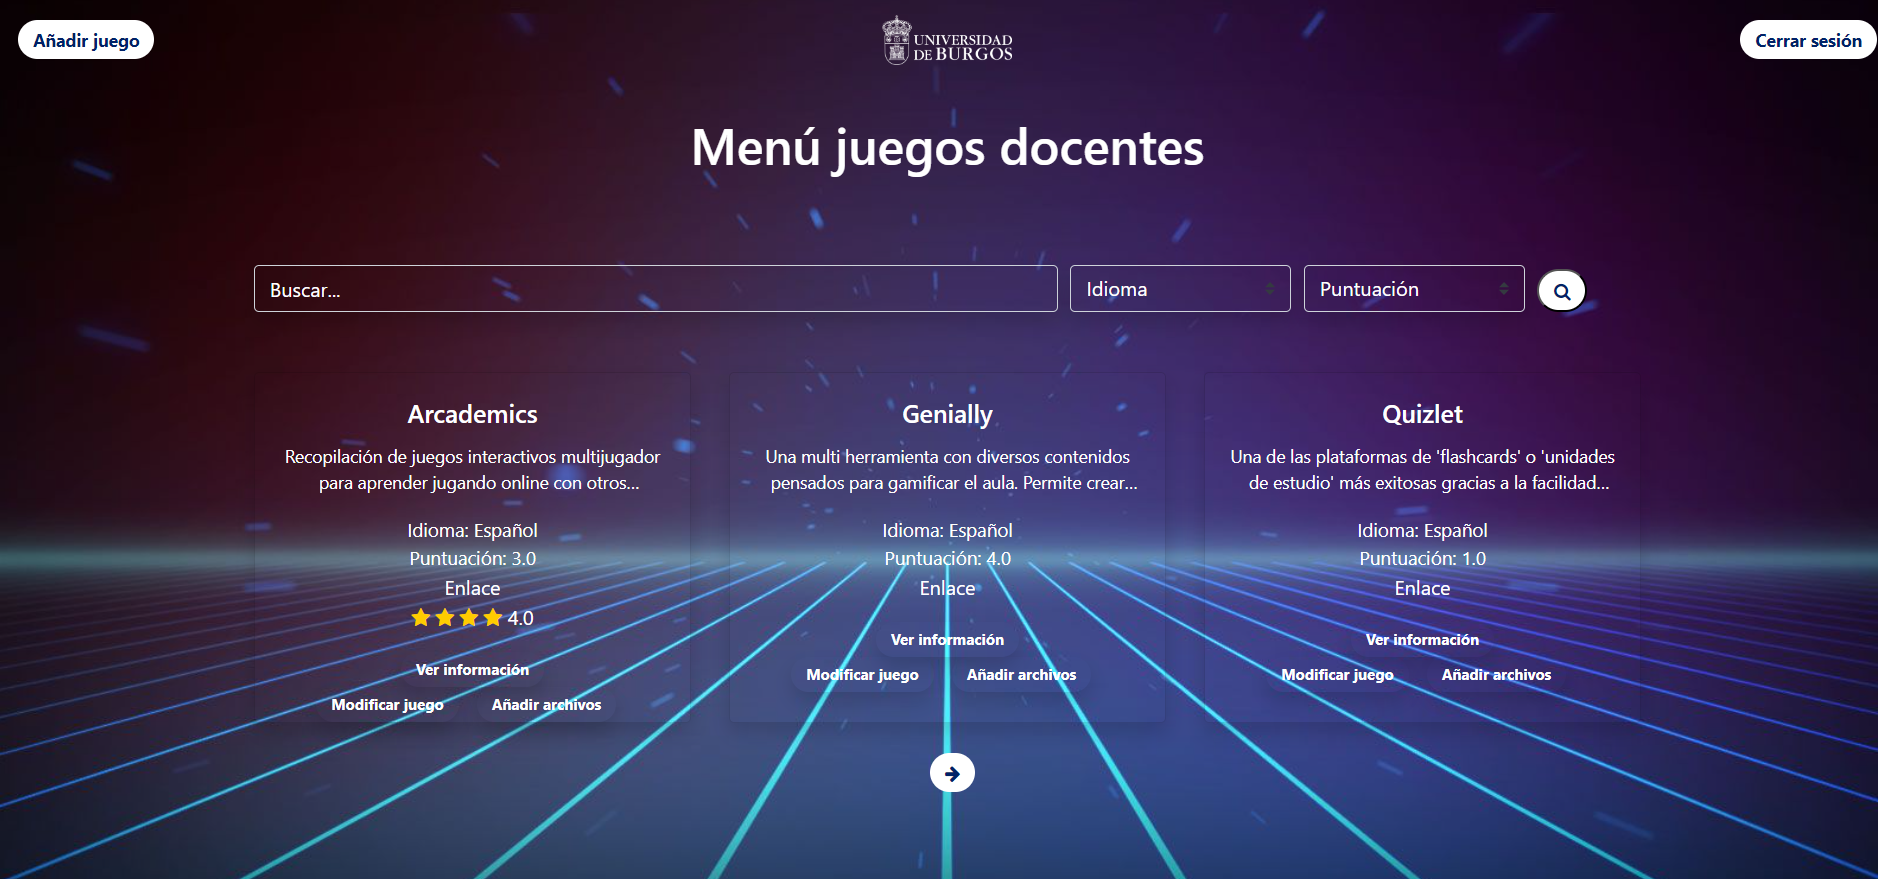
\includegraphics[width=1.0\textwidth]{menu-profesor}
\caption{Menú de juegos de profesores.}
\label{fig:menu-profesor}
\end{figure}

Al igual que el usuario, el profesor visualiza las tarjetas de información de los distintos juegos disponibles en la aplicación. 
\begin{figure}[htb]
\centering
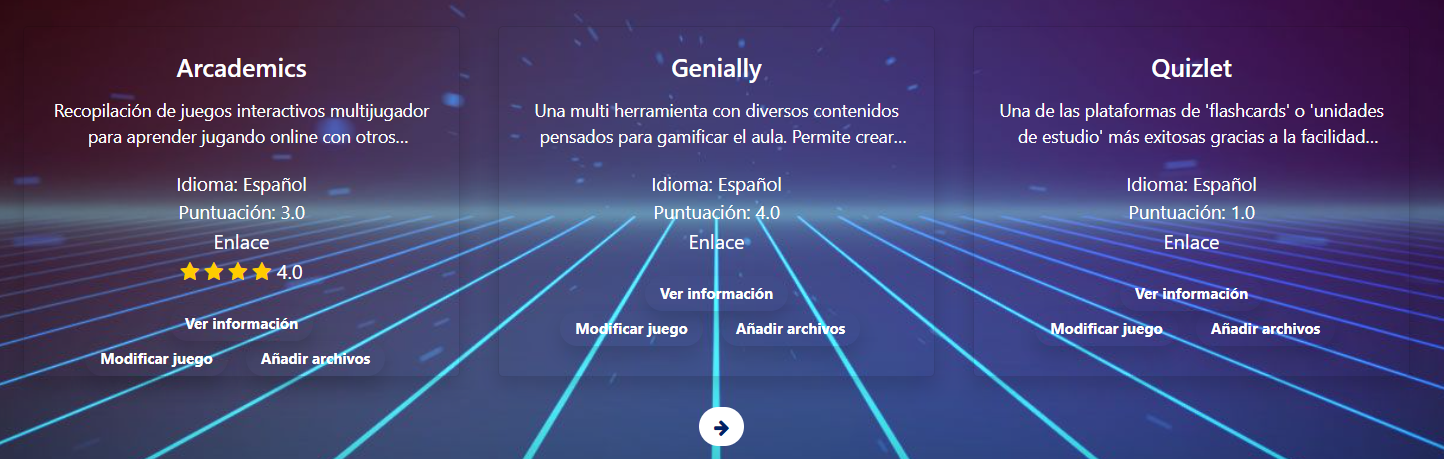
\includegraphics[width=1.0\textwidth]{tarjetas-profesor}
\caption{Tarjetas de juegos.}
\label{fig:tarjetas-profesor}
\end{figure}

Además, el profesor también dispone de una barra de búsqueda y filtros en la aplicación, lo que le permite realizar una búsqueda personalizada y más específica según sus intereses.
\newpage
\begin{figure}[htb]
\centering

\includegraphics[width=1.0\textwidth]{buscar}
\caption{Barra de búsqueda y filtros.}
\label{fig:buscar}
\end{figure}

Desde estas tarjetas, el profesor puede obtener más información sobre cada juego, modificar la información de los juegos existentes y añadir archivos relacionados a cada juego.
\begin{figure}[htb]
\centering
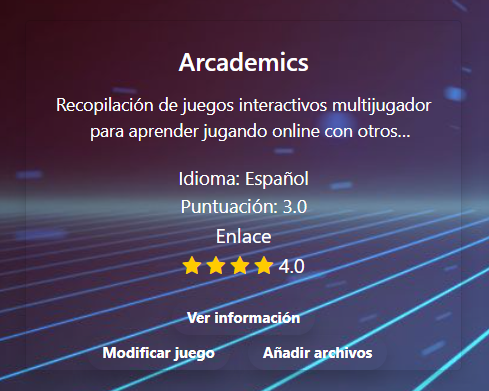
\includegraphics[width=0.5\textwidth]{btn-profe}
\caption{Botones para ver más información, modificar o añadir archivos.}
\label{fig:btn-profe}
\end{figure}

En la cabecera, el profesor también tiene acceso a un botón llamado ``Añadir juego``, a través del cual puede agregar un nuevo juego en la aplicación.

\begin{figure}[htb]
\centering

\includegraphics[width=0.2\textwidth]{btn-añadir}
\caption{Botón para añadir nuevo juego.}
\label{fig:btn-añadir}
\end{figure}

\subsection{Añadir un nuevo juego}
El profesor debe añadir toda la información requerida para añadir un nuevo juego.

\begin{figure}[htb]
\centering
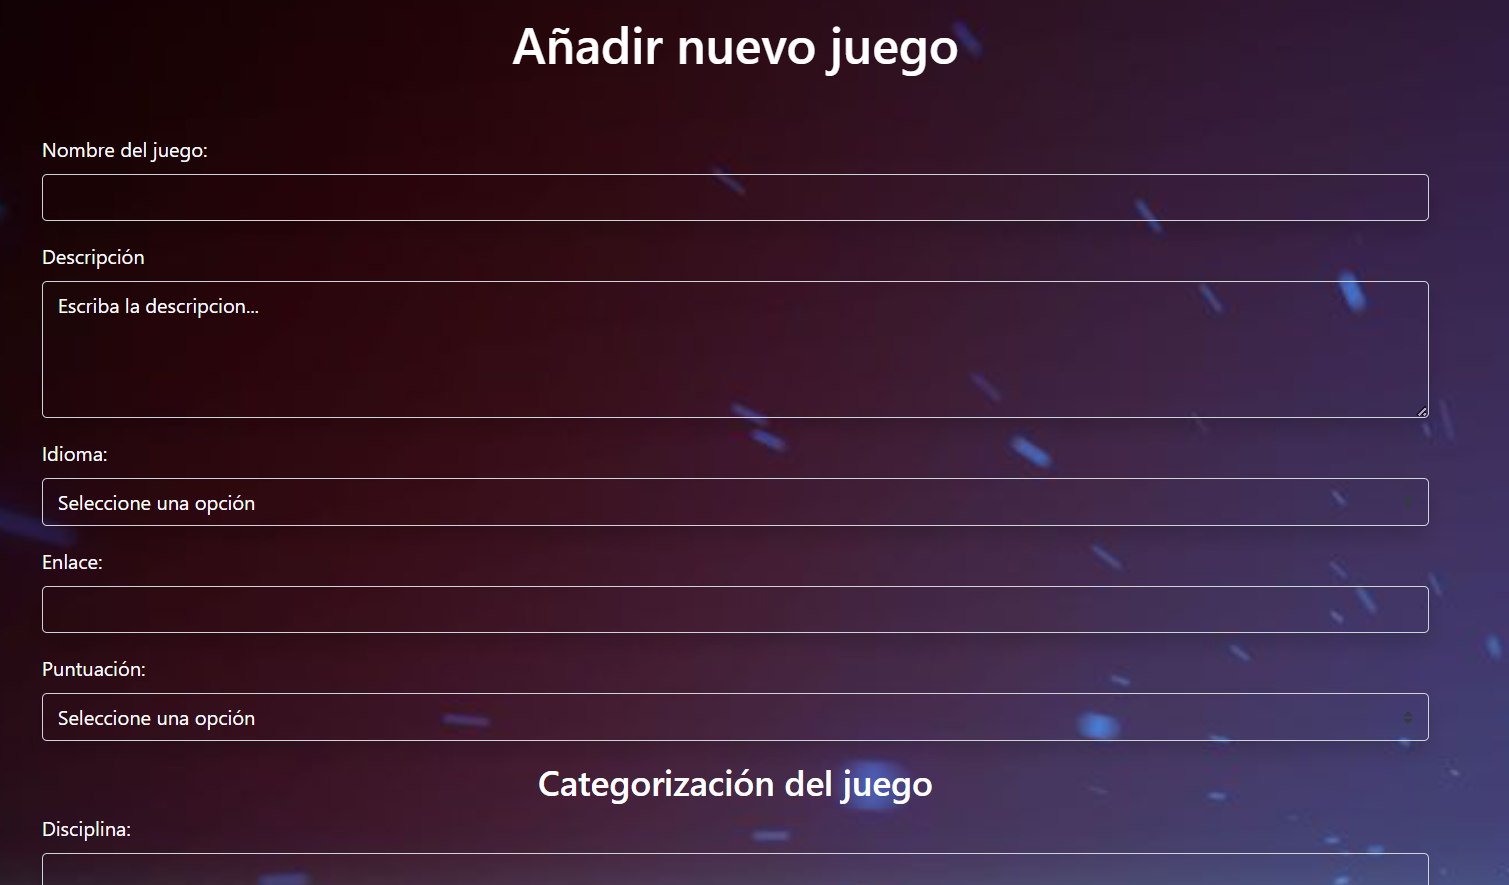
\includegraphics[width=0.8\textwidth]{nuevo-juego}
\caption{Añadir nuevo juego.}
\label{fig:nuevo-juego}
\end{figure}
\newpage
\subsection{Modificar un juego}
Se visualiza la información que contiene el juego que se va a modificar.
\begin{figure}[htb]
\centering
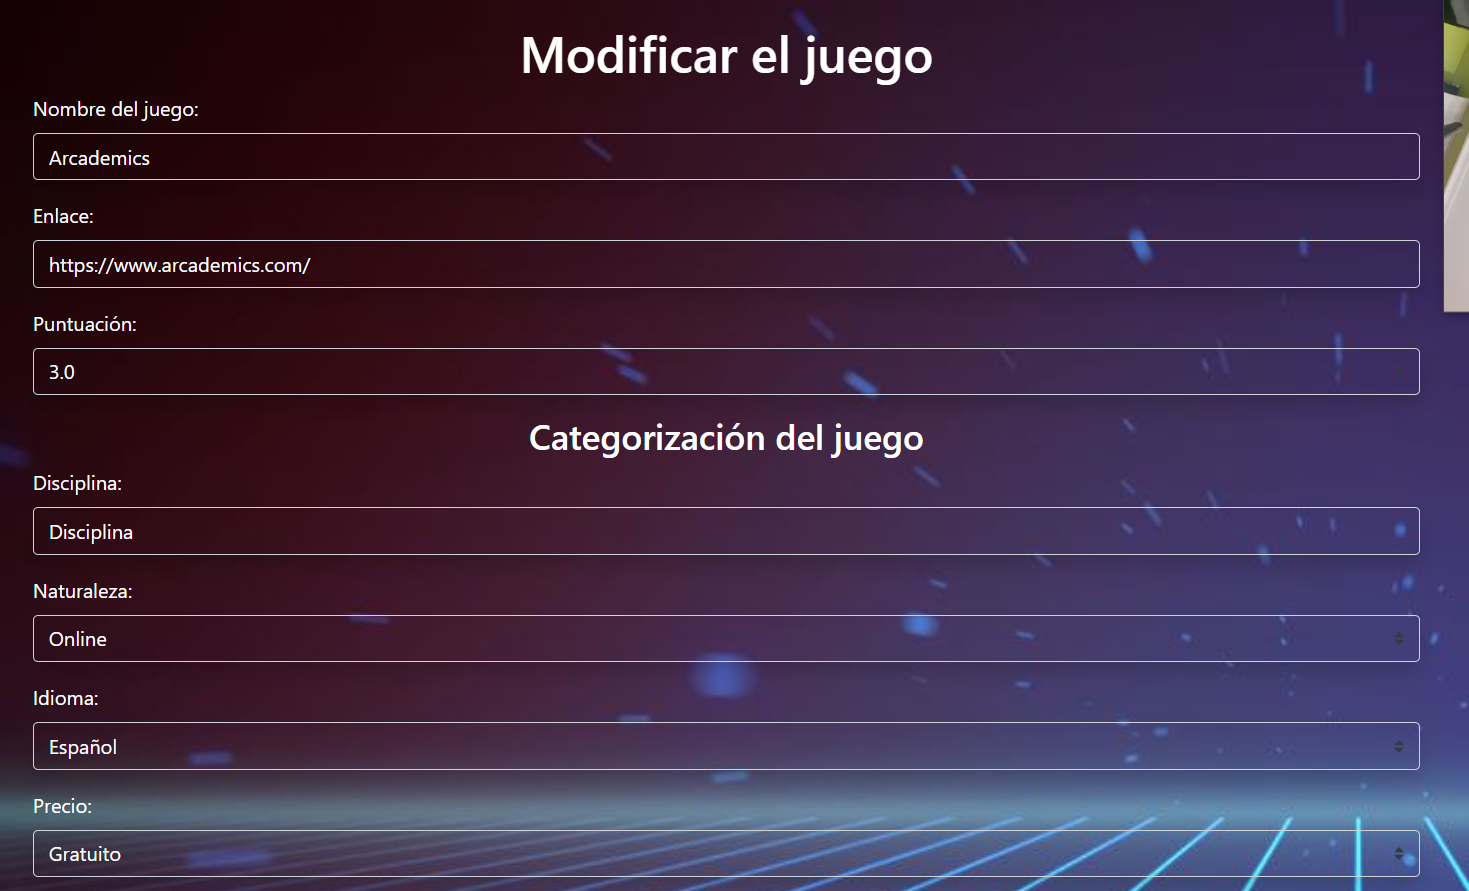
\includegraphics[width=0.8\textwidth]{juego-modificar}
\caption{Modificar juego.}
\label{fig:juego-modificar}
\end{figure}
\newpage

\subsection{Añadir archivos}
El profesor tiene la capacidad de añadir diferentes archivos para las instrucciones del jugador, las instrucciones del instructor y, si aplica, el archivo del juego.
\begin{figure}[htb]
\centering

\includegraphics[width=1.0\textwidth]{añadir-archivos}
\caption{Añadir archivos.}
\label{fig:añadir-archivos}
\end{figure}

En el caso de que se presione el botón de carga de archivos sin seleccionar ningún archivo, se mostrará un mensaje de error indicando que no se ha seleccionado ningún archivo.
\begin{figure}[htb]
\centering

\includegraphics[width=1.0\textwidth]{error-no-archivo}
\caption{Error no se seleccionó el archivo.}
\label{fig:error-no-archivo}
\end{figure}

Si el usuario intenta cargar un archivo que excede el límite de tamaño establecido, se mostrará una alerta que impide la carga del archivo.
\newpage
\begin{figure}[htb]
\centering
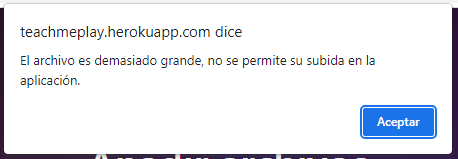
\includegraphics[width=0.6\textwidth]{error-tamaño}
\caption{Alerta error de tamaño.}
\label{fig:error-tamaño}
\end{figure}

Si el usuario intenta cargar un archivo con un tipo de archivo no válido, también se mostrará un mensaje de error que impide la carga del archivo y se informará al usuario sobre los tipos de archivo permitidos.
\begin{figure}[htb]
\centering
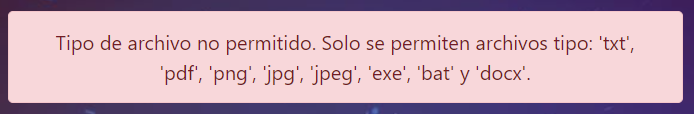
\includegraphics[width=1.0\textwidth]{error-tipo}
\caption{Error de tipo.}
\label{fig:error-tipo}
\end{figure}

También se tiene en cuenta la longitud del nombre del archivo, por lo que si el usuario intenta cargar un archivo con un nombre demasiado largo saldrá un error.
\begin{figure}[htb]
\centering

\includegraphics[width=1.0\textwidth]{error-nombre}
\caption{Error de nombre.}
\label{fig:error-nombre}
\end{figure}

En caso de que el archivo que el usuario intenta cargar cumpla todas las restricciones establecidas, se mostrará un mensaje de éxito y se realizará la carga del archivo. Sin embargo, es importante tener en cuenta que esta funcionalidad solo estará disponible en la máquina virtual de prueba, ya que en la aplicación desplegada se generará un error al intentar cargar archivos.
\begin{figure}[htb]
\centering

\includegraphics[width=1.0\textwidth]{archivo-exito}
\caption{Archivo cargado con éxito.}
\label{fig:archivo-exito}
\end{figure}

\subsection{Menú de juegos para el administrador}
Cuando el administrador ha iniciado sesión correctamente, se le redirige a su menú de juegos, donde puede acceder a diversas funcionalidades.
\begin{figure}[htb]
\centering
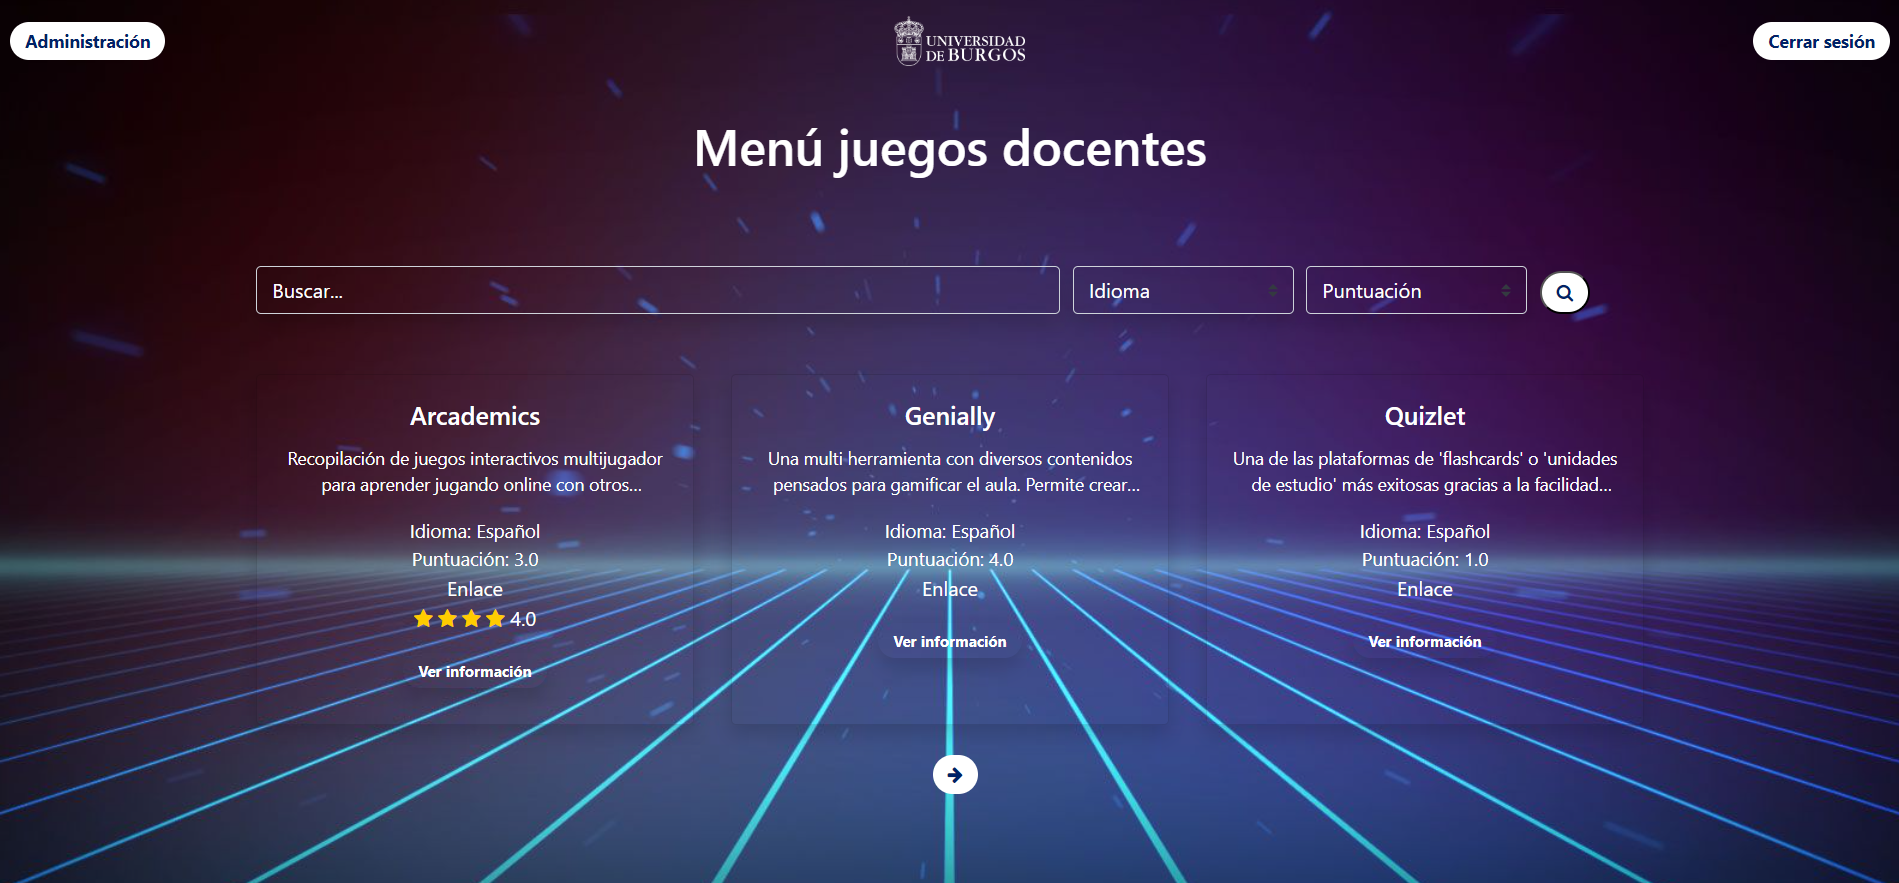
\includegraphics[width=1.0\textwidth]{menu-administrador}
\caption{Menú de juegos del administrador.}
\label{fig:menu-administrador}
\end{figure}

Al igual que el usuario y el profesor, el administrador visualiza las tarjetas de información de los distintos juegos disponibles en la aplicación. Además, el administrador también dispone de una barra de búsqueda y filtros en la aplicación, lo que le permite realizar una búsqueda personalizada y más específica según sus intereses.

En la cabecera, el administrador tiene acceso a un botón llamado ``Administración``, a través del cual puede gestionar los juegos, usuarios y solicitudes.

\begin{figure}[htb]
\centering

\includegraphics[width=0.2\textwidth]{btn-administracion}
\caption{Botón de administración.}
\label{fig:btn-administracion}
\end{figure}

\subsection{Administración}
Al pulsar el botón de administración se visualiza un panel para la administración de juegos, usuarios y solicitudes.
\begin{figure}[htb]
\centering
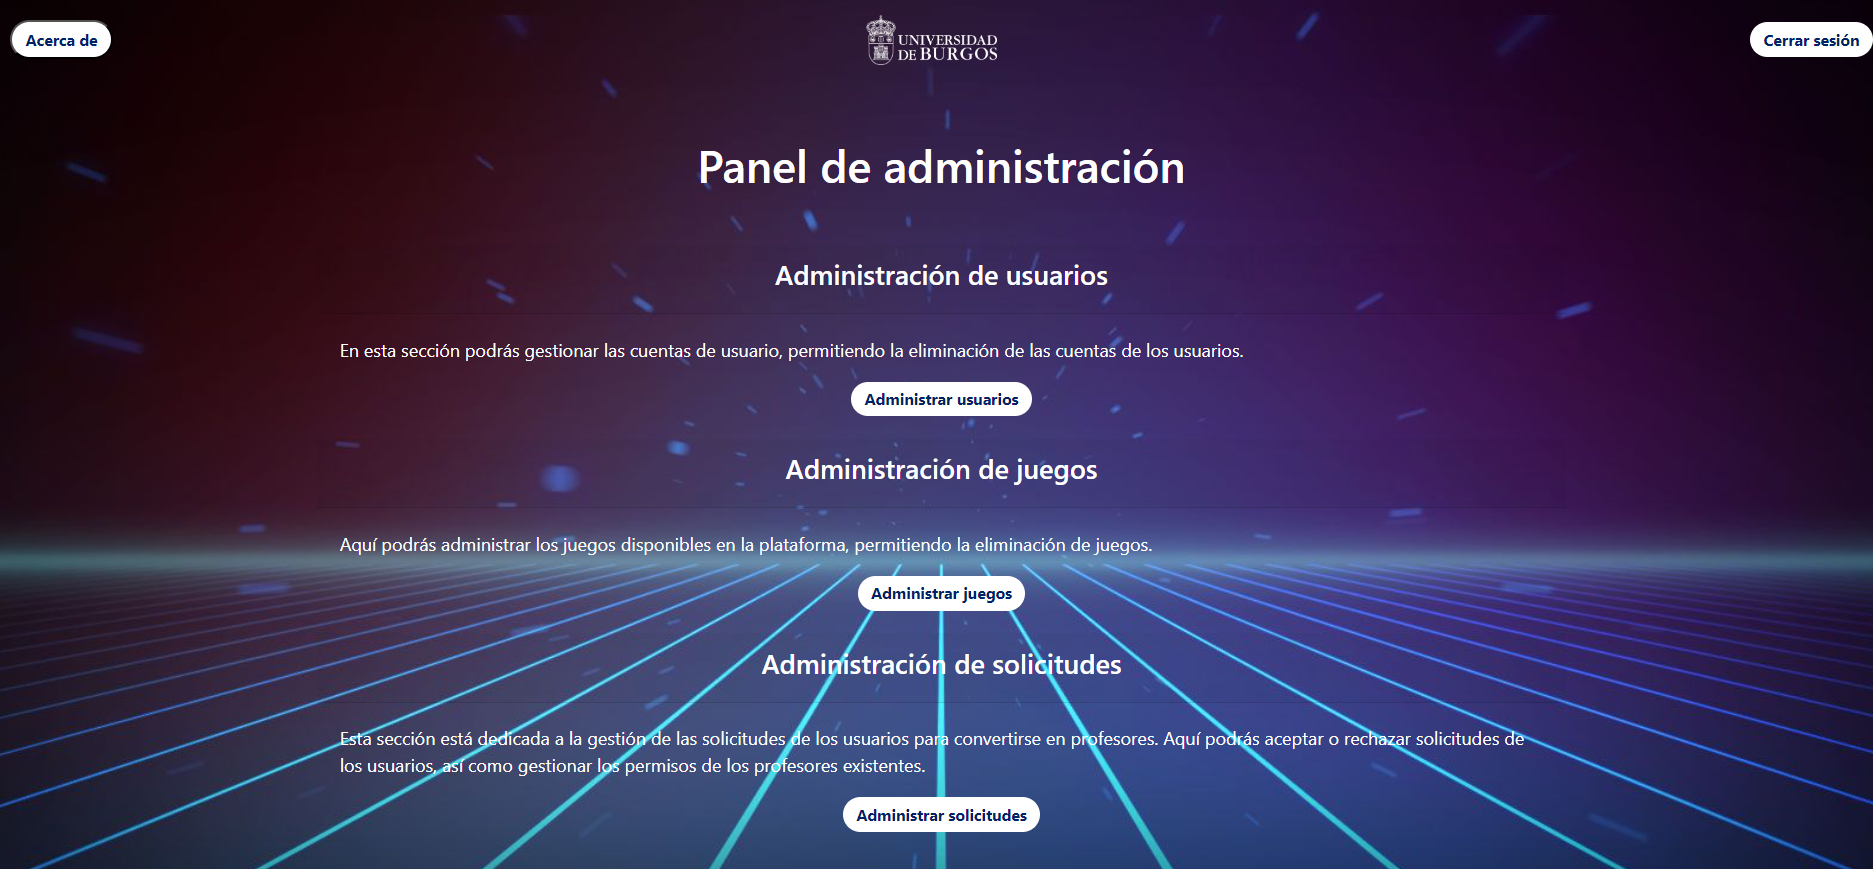
\includegraphics[width=1.0\textwidth]{administracion}
\caption{Botón de administración.}
\label{fig:administracion}
\end{figure}

Desde la gestión de juegos, el administrador puede ver los juegos que se encuentran en la aplicación y tiene la opción de eliminarlos.
\begin{figure}[htb]
\centering

\includegraphics[width=1.0\textwidth]{eliminar-juegos}
\caption{Eliminar juegos.}
\label{fig:eliminar-juegos}
\end{figure}
\newpage
Desde la gestión de usuarios, el administrador puede ver la lista de usuarios registrados en la aplicación y tiene la opción de eliminarlos.

\begin{figure}[htb]
\centering
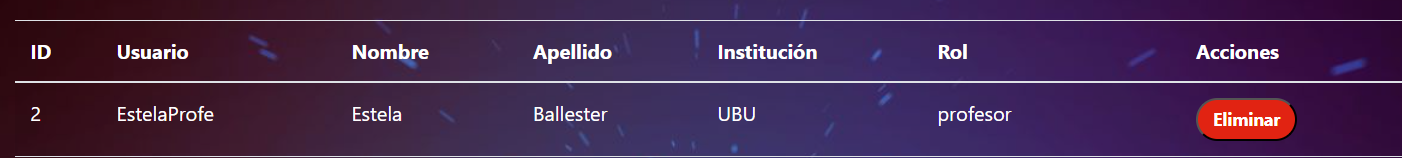
\includegraphics[width=1.0\textwidth]{eliminar-usuarios}
\caption{Eliminar usuarios.}
\label{fig:eliminar-usuarios}
\end{figure}

Desde la gestión de solicitudes, el administrador puede visualizar las solicitudes pendientes y aprobarlas.
\begin{figure}[htb]
\centering
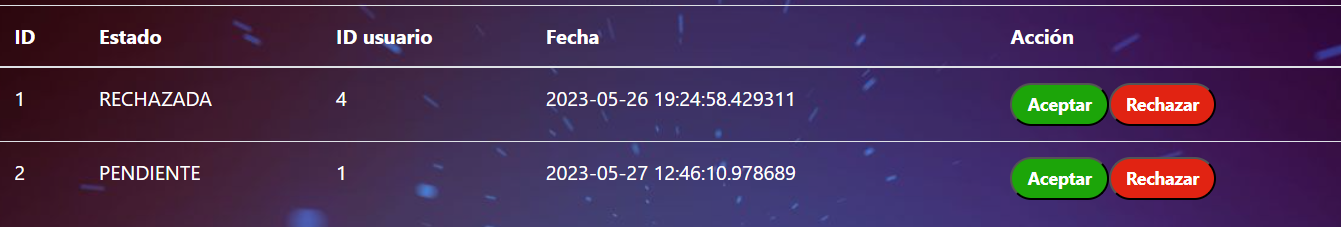
\includegraphics[width=1.0\textwidth]{solicitudes}
\caption{Aceptar o rechazar solicitudes.}
\label{fig:solicitudes}
\end{figure}